\begin{figure*}[t]
\small
\setlength{\tabcolsep}{3pt}
\centering
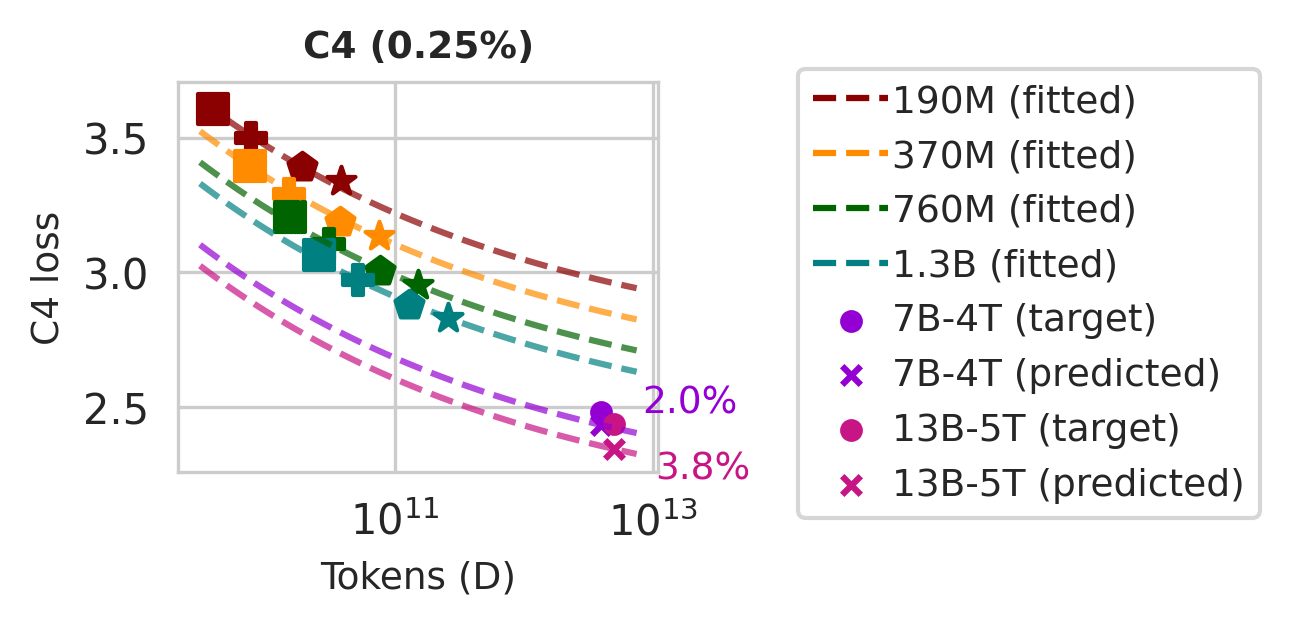
\includegraphics[width=0.5 \linewidth]{images/step1_c4_main.png}
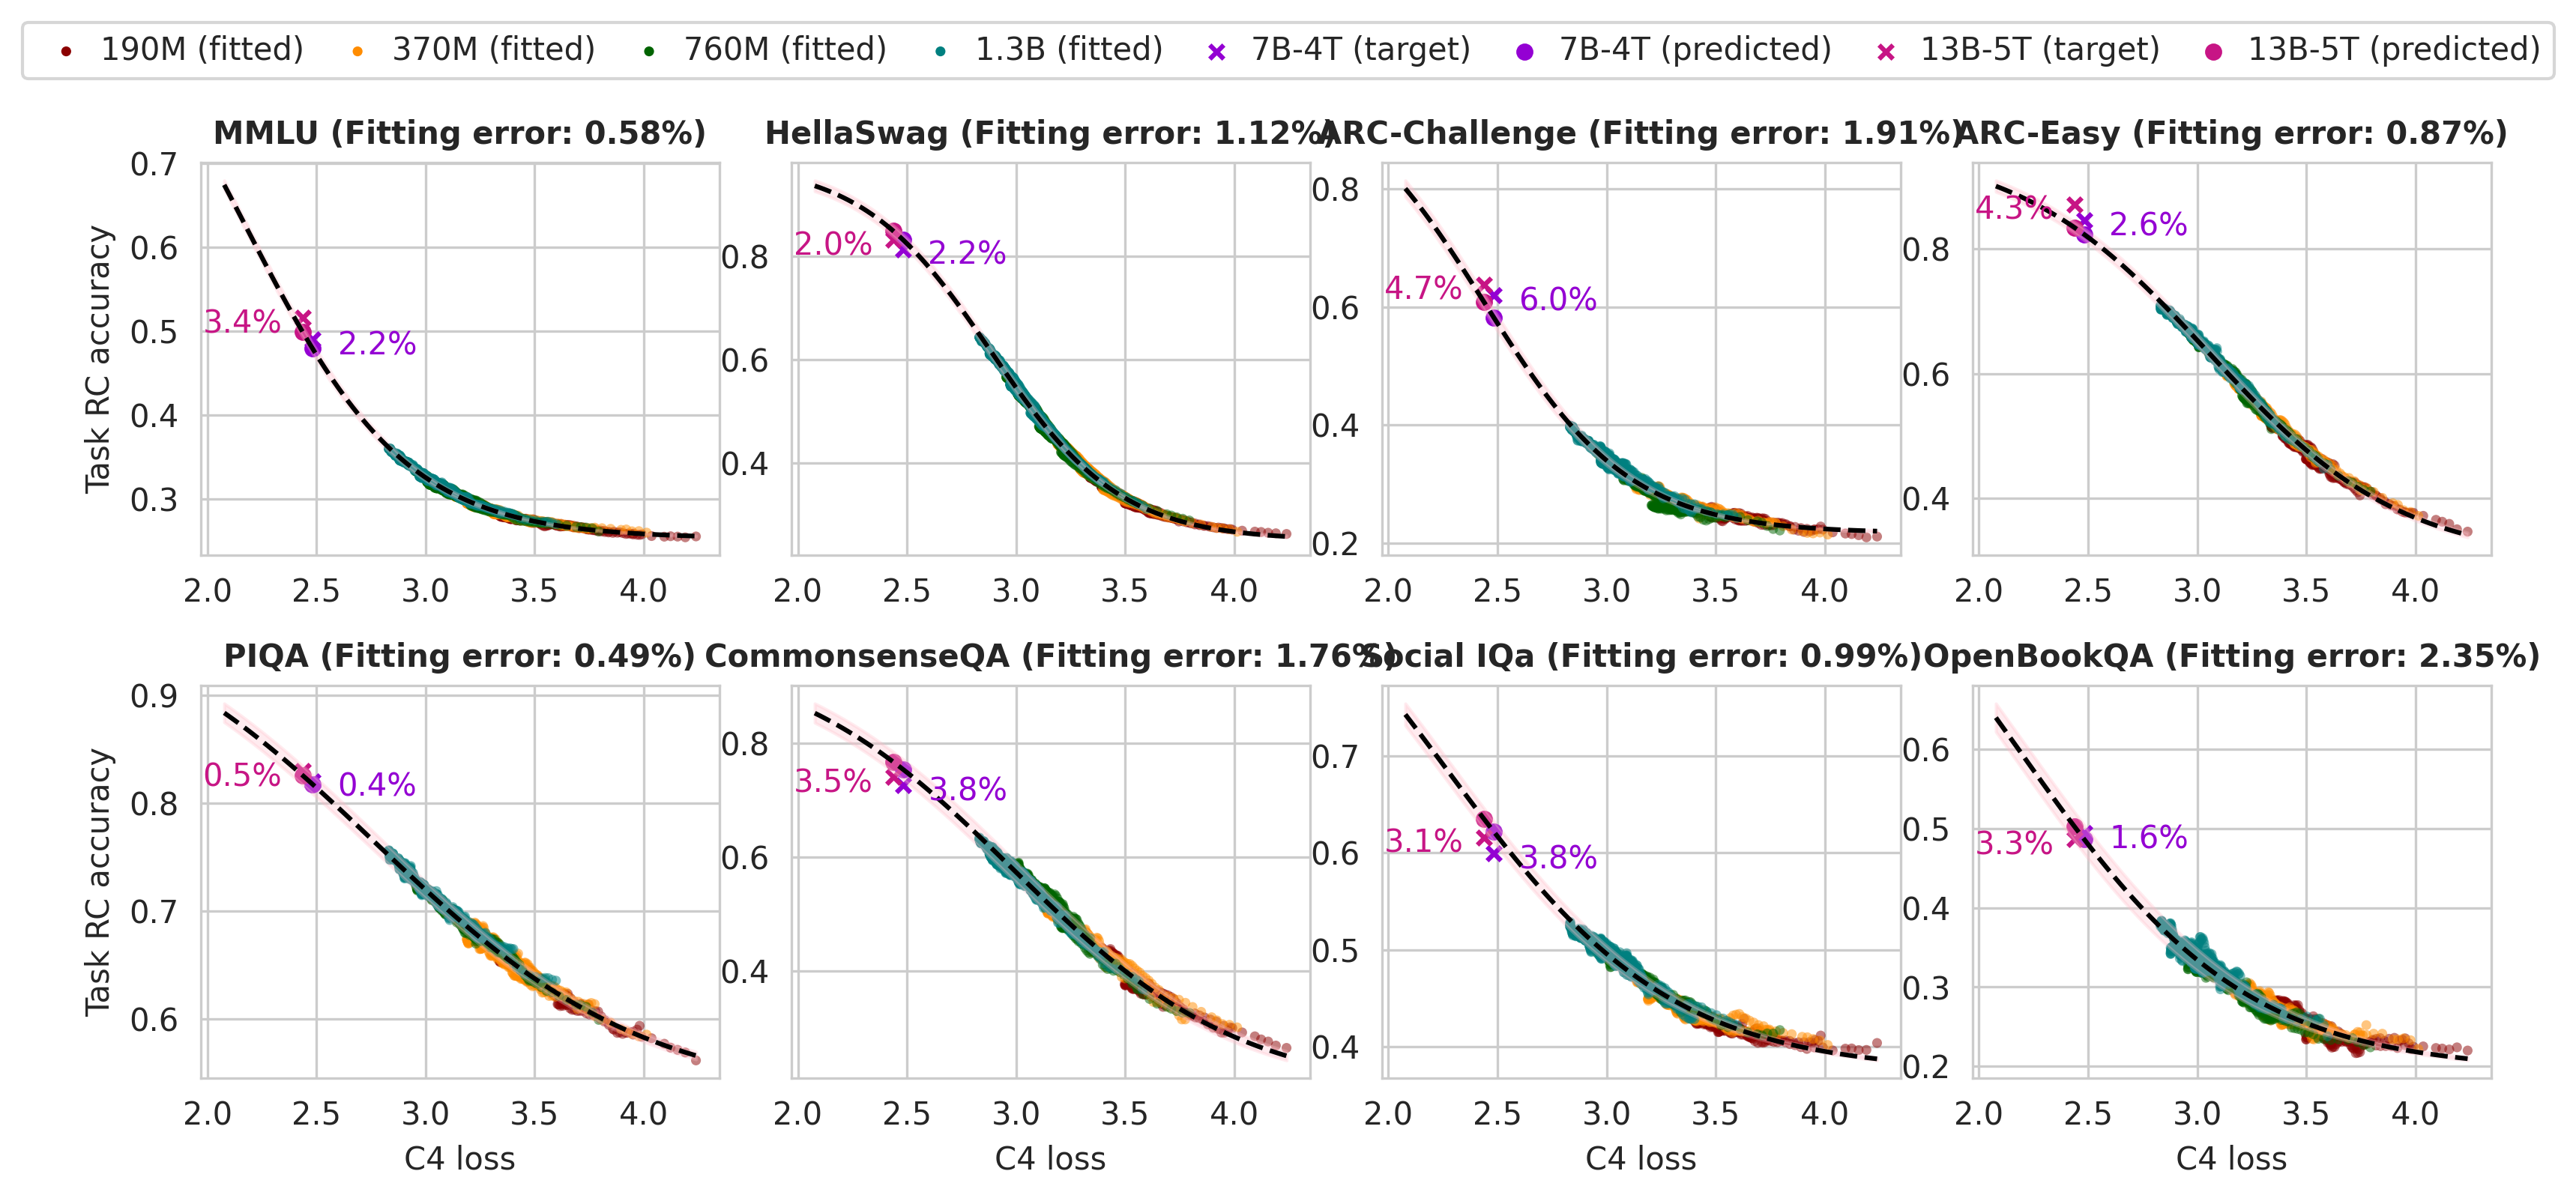
\includegraphics[width=\linewidth]{images/step2_c4_main.png}
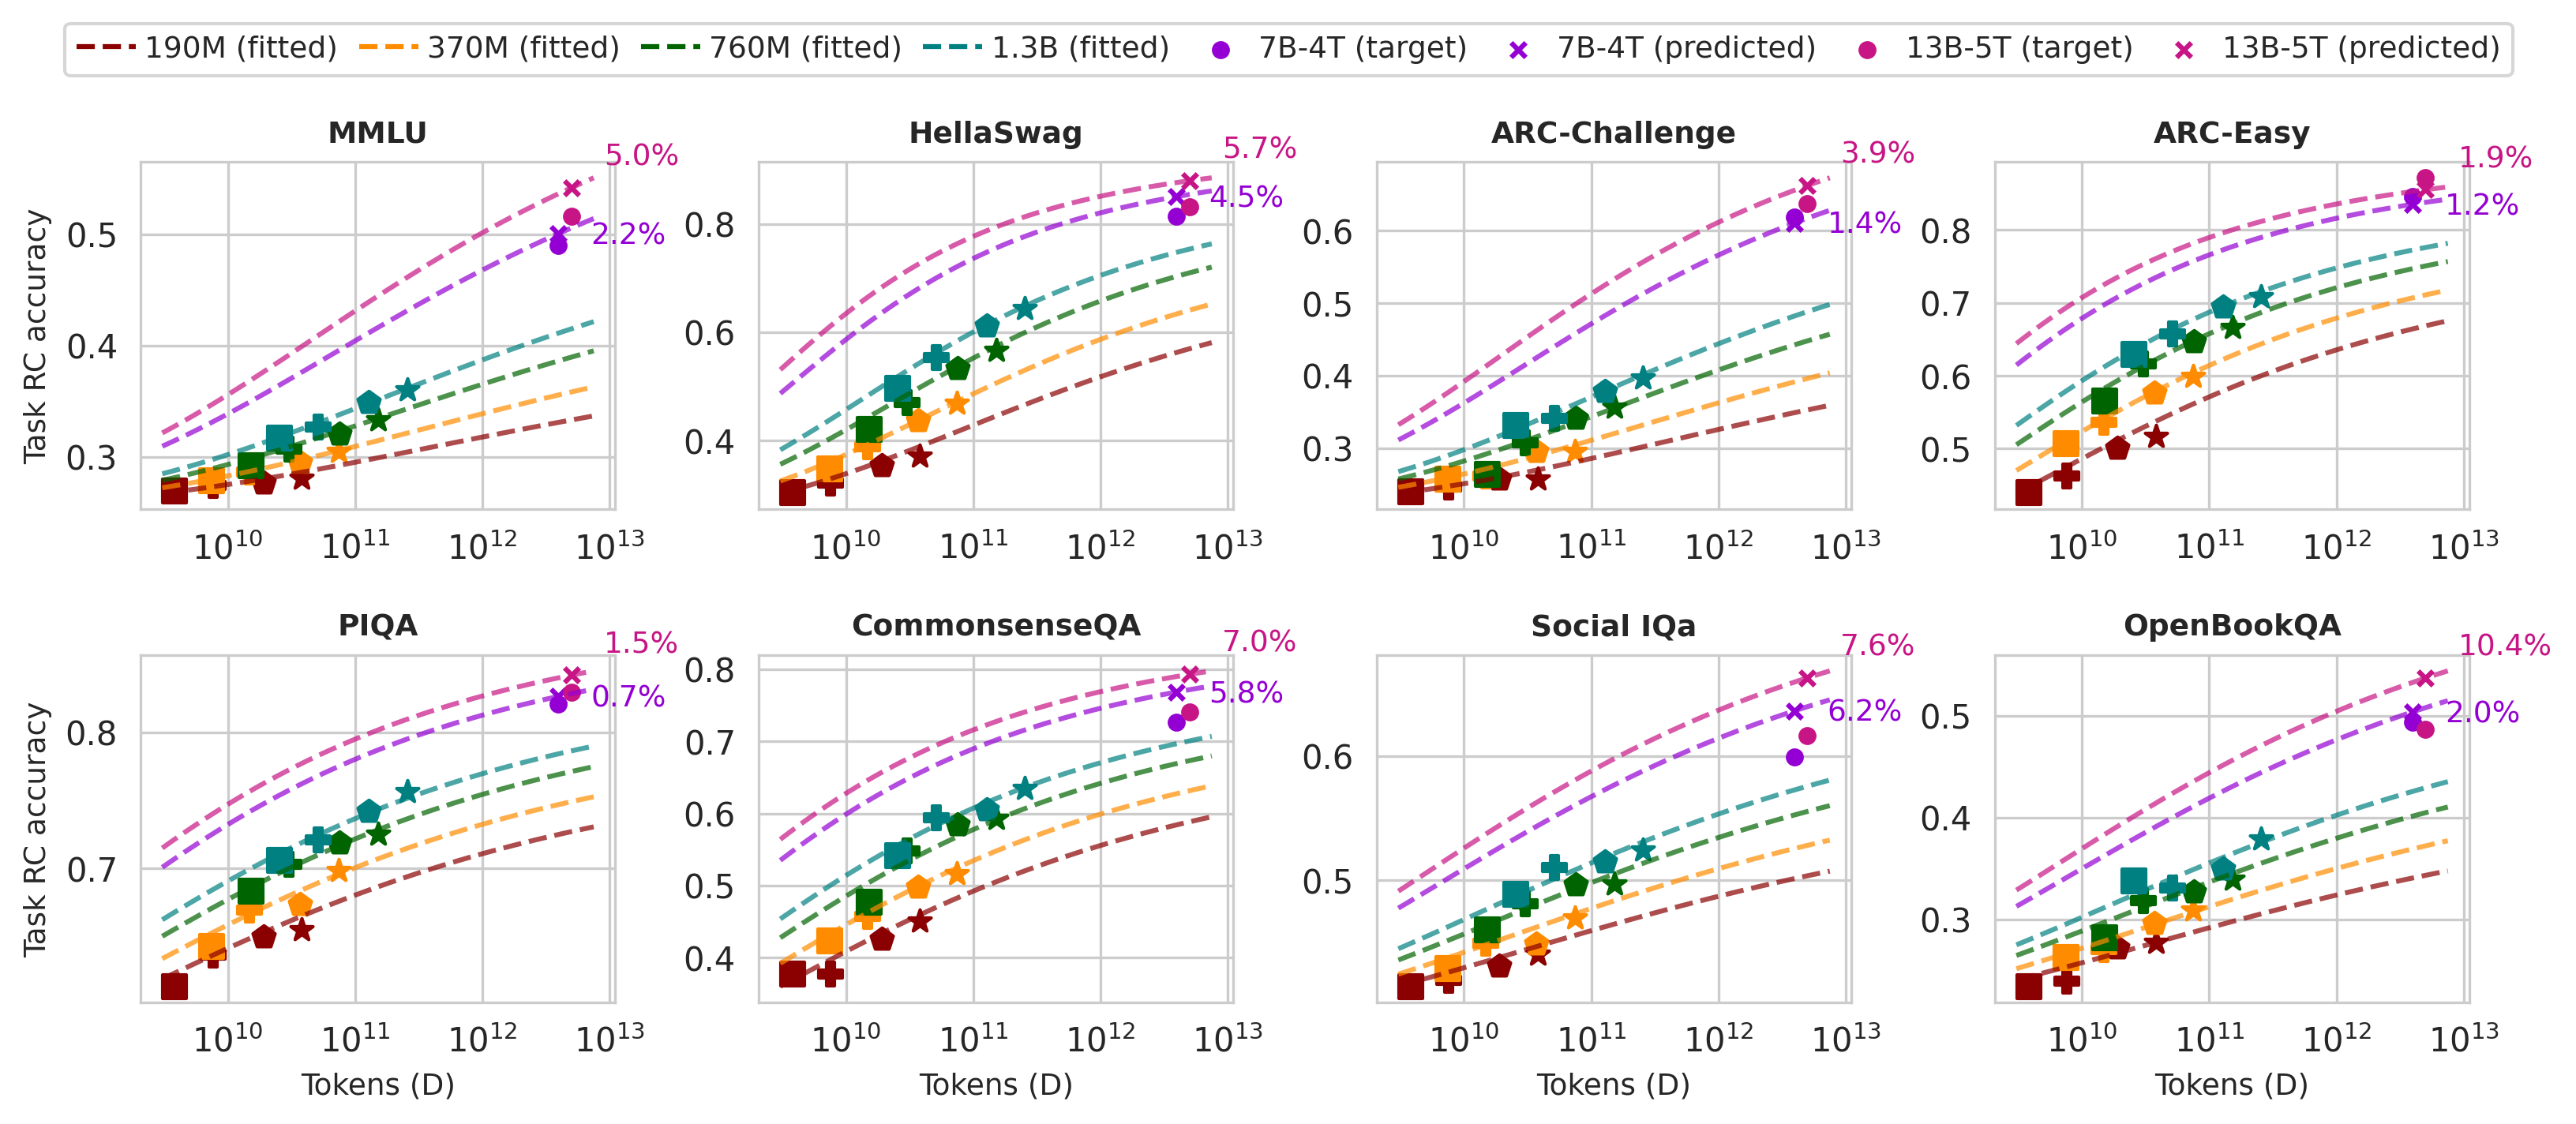
\includegraphics[width=\linewidth]{images/chained_c4_main.png}
% \begin{tabular}{c l | r r r r | r r r r}
% \toprule
% & & \multicolumn{4}{c|}{\textbf{7B-4T}} & \multicolumn{4}{c}{\textbf{13B-5T}} \\
% & & Pred & Actual & Error & \%Error & Pred & Actual & Error & \%Error \\
% \midrule
% \multirow{8}{*}{\textbf{RC}} & MMLU & 50.1 & 49.0 & 1.1 & 2.2\% & 54.2 & 51.6 & 2.6 & 5.0\% \\
% & HellaSwag & 85.0 & 81.3 & 3.7 & 4.5\% & 87.9 & 83.2 & 4.7 & 5.7\% \\
% & ARC-Challenge & 61.1 & 61.9 & 0.8 & 1.4\% & 66.3 & 63.8 & 2.5 & 3.9\% \\
% & ARC-Easy & 83.5 & 84.6 & 1.1 & 1.2\% & 85.5 & 87.2 & 1.7 & 1.9\% \\
% & PIQA & 82.6 & 82.0 & 0.6 & 0.7\% & 84.2 & 83.0 & 1.2 & 1.5\% \\
% & CommonsenseQA & 76.8 & 72.6 & 4.2 & 5.8\% & 79.3 & 74.1 & 5.2 & 7.0\% \\
% & Social IQa & 63.6 & 59.9 & 3.7 & 6.2\% & 66.3 & 61.6 & 4.7 & 7.6\% \\
% & OpenBookQA & 50.4 & 49.4 & 1.0 & 2.0\% & 53.7 & 48.6 & 5.1 & 10.4\% \\
% \bottomrule
% \end{tabular}
\caption{
    Using language modeling loss on C4-en validation as the intermediate feature.
    \textbf{From top to bottom}: step 1, step 2, and chaining the two steps.
}
\label{fig:c4}
% \vspace{-16pt}
\end{figure*}